
\begin{figure*}
\centering
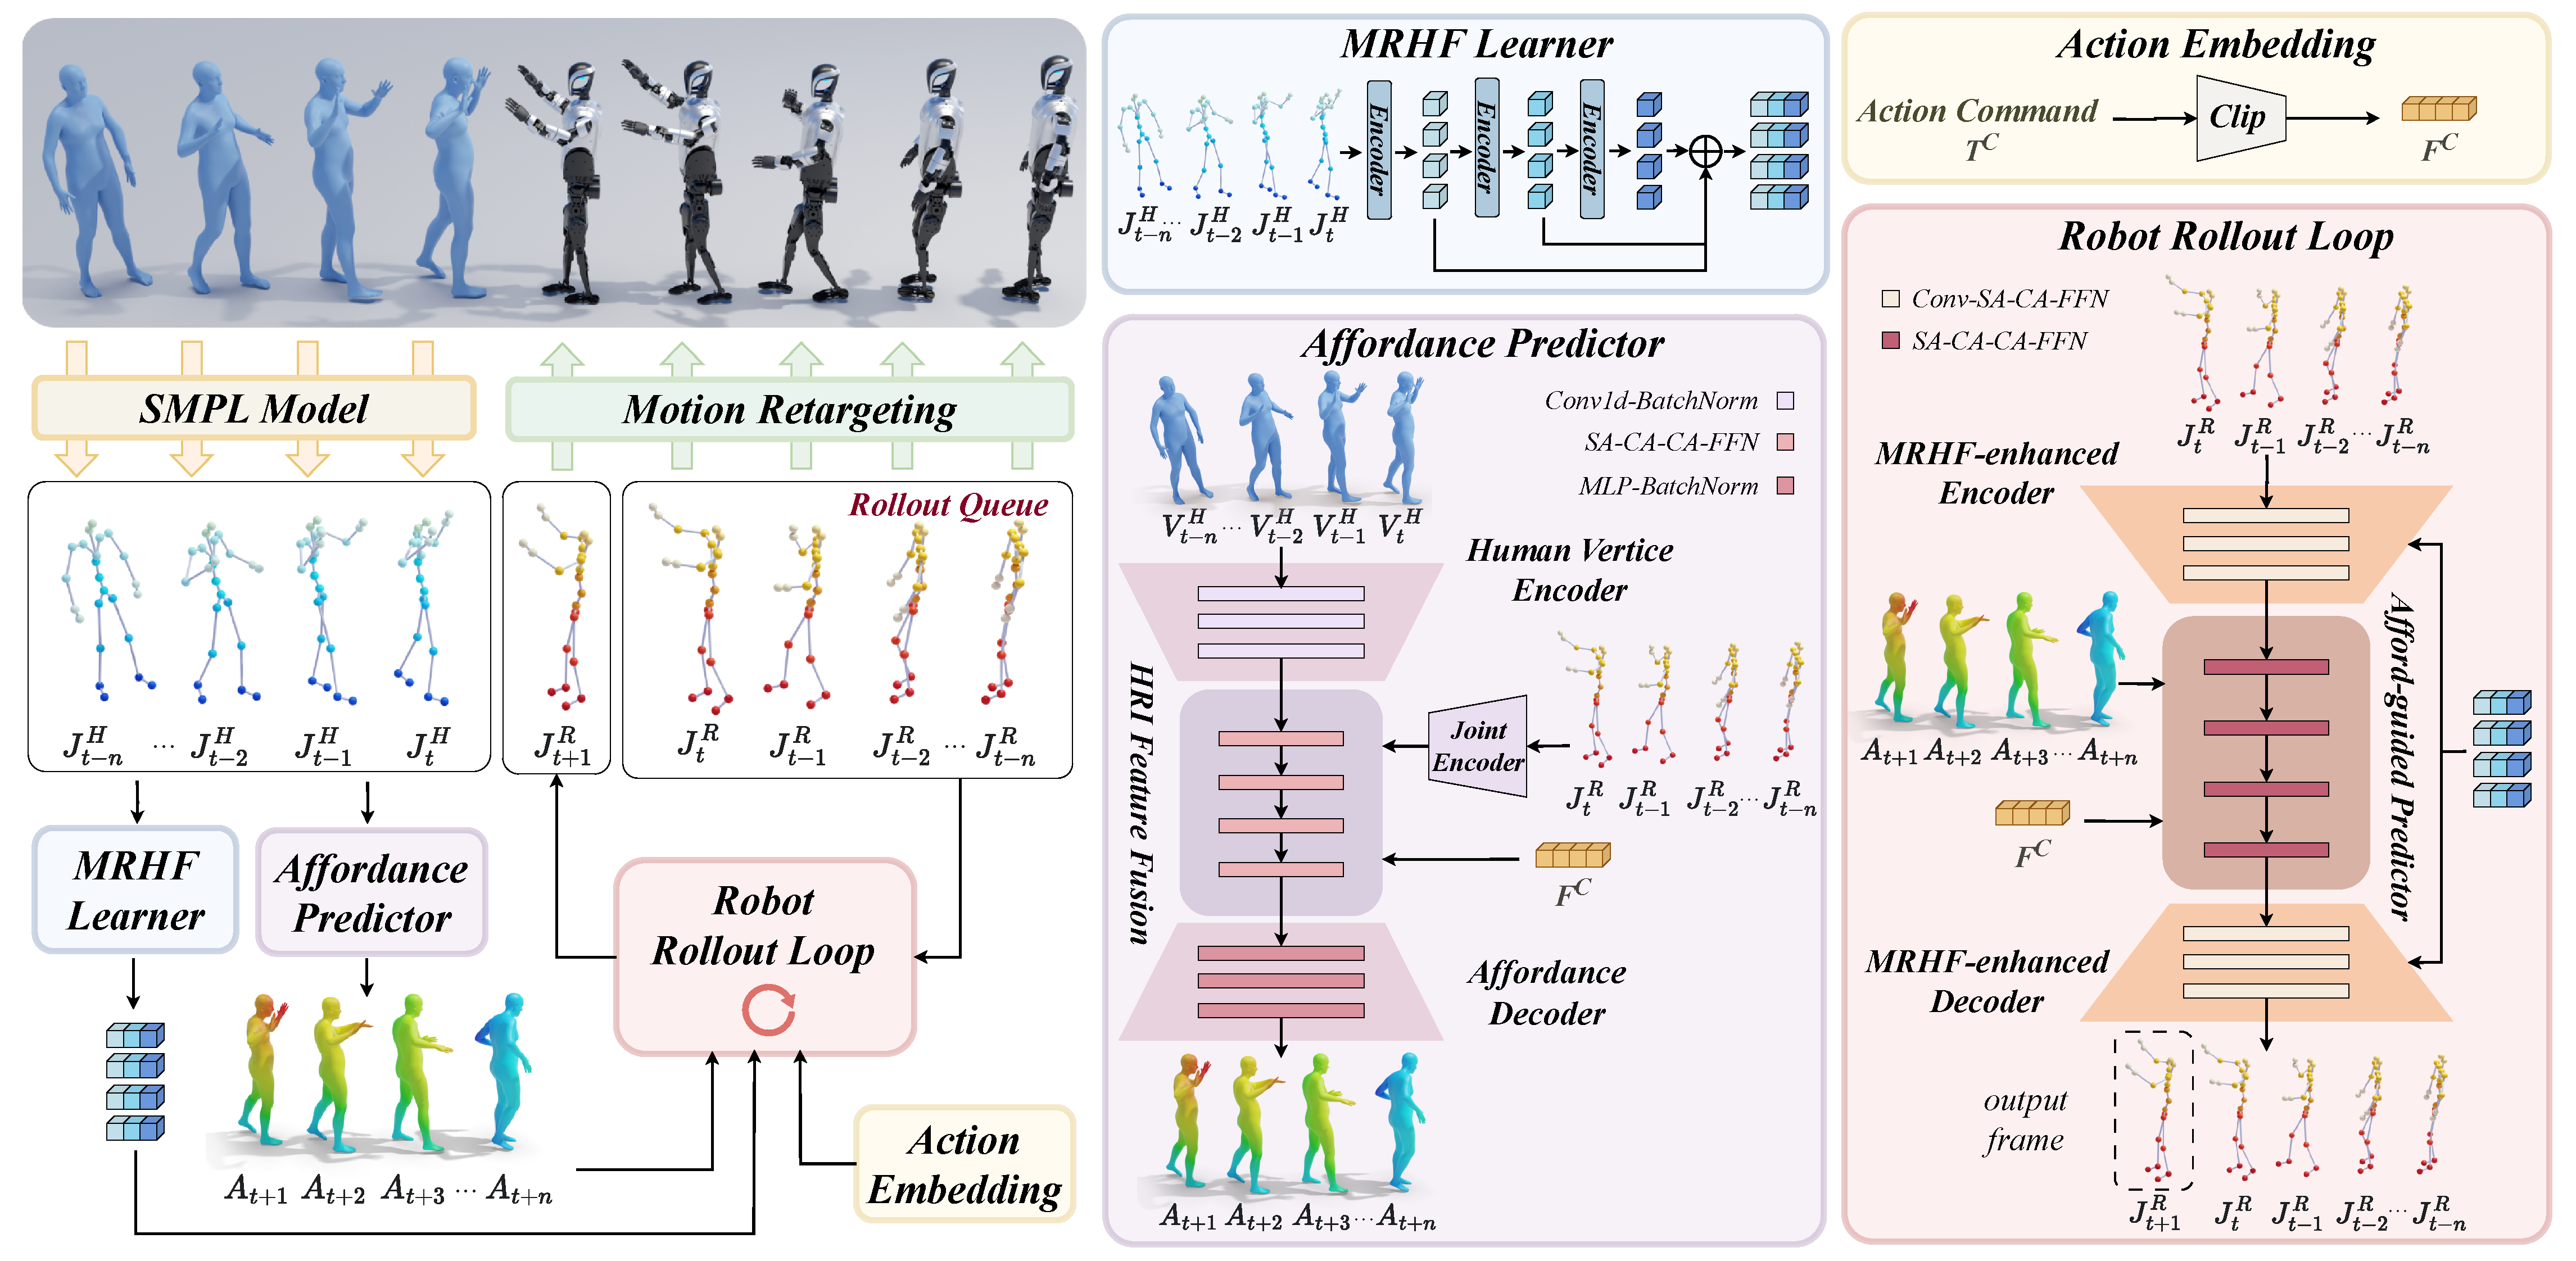
\includegraphics[width=1\linewidth]{images/intermodel-mainv5.pdf}
\vspace{-20pt}
\caption{Overall pipeline of our Robotic Interaction Model. The model ingests text action commands, historical robot joints, observed human joints and SMPL mesh vertices, and processes them through four tightly coupled modules. The Affordance Predictor explicitly estimates dense end-effector–vertex spatial fields to enable dexterous, socially-appropriate contact reasoning; the Multi-Resolution Human Feature (MRHF) Learner fuses hierarchical temporal cues to boost situational awareness; the Robot Rollout Loop leverages these affordance and human features to iteratively generate coherent, context-adaptive joint trajectories for real-time responsiveness; and finally, the Motion Retargeting module maps each predicted skeleton frame to robot-specific angle axis.}
\label{fig:interactiveModel}
\vspace{-10pt}
\end{figure*}
\section{Design Goals}

Towards the human-robot symbiosis, our primary purpose is to develop a human-in-the-loop system that supports the versatile interactions between humans and robots, such as hand-shaking, hugging, etc. In this way, human users can easily obtain more experiences to get used to interacting with robots and returning their authentic feedback to improve robot skills to better facilitate human life. We decompose it into specific design goals as follows.

\noindent\textbf{D1. Simulate a realistic and real-time human-robot interaction experience.} To allow human users to interact with virtual robots, the system must capture human motion, produce a robot reaction, and present it to the user. More importantly, the whole pipeline should be realistic and real-time enough for the user to have an immersive experience like interacting in the real world.

\noindent\textbf{D2. Produce reasonable and plausible robot reactions regarding human behavior.} 
Humans may perform various actions during interactions. The fundamental capability of the system is to automatically determine the appropriate robot reaction based on human behavior to ensure a fluent human-robot interaction.

\noindent\textbf{D3. Facilitate human feedback collection for robot interaction skill enhancement.} Over the long-term interactions, humans and robots should mutually adapt to each other to achieve harmonious co-existence. It requires an efficient fine-tuning mechanism to continuously enhance the robot's interaction skills. Therefore, the system should facilitate the collection of human-robot interaction data with authentic human feedback and efficiently utilize the collected data to fine-tune robot interactions.

\section{Symbridge System}
\subsection{System Architecture}

The aforementioned design goals lead to our system architecture, as illustrated in Fig.~\ref{fig:system}. The core is the immersive human-robot interaction with our AR interface, where a human user can wear AR glasses to interact with the virtual robot in the real environment. It activates the two main capabilities of our system.


The \emph{human-robot interaction}, illustrated with the blue arrows in Fig.~\ref{fig:system}, aims to support the realistic and real-time interactions between humans and the virtual robot. First, the human behavior is continuously acquired as motion sequences by the motion capture module. Given the current frame and the cached historical frames of the captured human motion, we employ an interactive model to predict the next frames of the robot motion. The predicted robot motion is sent %to the physical simulation module, which leverages a physical humanoid controller to infer the physically feasible robot reactions that align with the predicted robot motion as much as possible. Finally, the simulated robot poses are transmitted 
to the applications running on the AR glasses to provide immersive interaction experiences. Our system also provides a third-person perspective by presenting the captured real human and rendered virtual robot on the same visual frame.

The \emph{model adaptation}, illustrated with the yellow arrows in Fig.~\ref{fig:system}, aims to enhance the robot's interaction skills by collecting and utilizing the human-in-the-loop interaction data. During the human-robot interaction through the AR interface, the human users may express their feedback, such as ratings on the quality of interaction experiences. Our system records the interaction process as well as the human feedback, and utilizes them to fine-tune the interactive model to adapt it to human preference. %After fine-tuning, the interactive model is updated to further assist the human-robot interactions. 

\subsection{Modules for Human-Robot Interaction}
\label{sec:mocap}
%To facilitate realistic and real-time human-robot interaction, the platform should capture human motions to mimic robot perception and present the robot reactions to the user. They can be considered as providing the input and processing the output of a pluggable \textbf{Robotic Interaction Model}, which will be introduced in Section~\ref{sec:interactivemodel}.

\noindent\textbf{Motion Capture.} To enable realistic and real-time human–robot interaction, the system requires accurate motion capture that approximates the robot’s perception. We employ an Ouster OS1-128 LiDAR sensor to acquire 3D point clouds of the human subject. This device provides high-precision depth information while inherently preserving user privacy by not capturing appearance textures. Moreover, it operates robustly under varying lighting conditions. In our setup, the LiDAR is positioned in front of the user, who can move within a range of 5–7 meters from the sensor.
Then, we employ the cutting-edge LiDAR-based framework LiveHPS++~\cite{ren2025livehps++}, which estimates pose parameters of human motions from scanned point clouds. More details are in supplementary material. %During the interactions, we set a 10FPS speed of the motion capture system due to the limit of the LiDAR device.

%\noindent\textbf{Interactive Model.} Given the human pose parameters from the motion capture module, we first convert them into joint positions of the human body skeleton with a forward kinematic algorithm. Then, for every frame, the interactive model takes historical and current human poses and robot poses, as well as the user's action command such as "handshake" as input, and outputs a sequence of the predicted \color{red}next \color{black} robot poses. All the input and output poses of the interactive model are represented as the joint positions of the skeletons, either of a human or a robot body, \color{red}for ...\color{black} After that, we further convert the output robot pose via an online inverse kinematics solver. [Why include these FK and IK? One can also ...]

%\noindent\textbf{Physical Simulation.} We employ the deep reinforcement learning technique presented in~\cite{luo2023perpetual} to control simulated robots in a physical simulation environment, i.e., IssacGym~\cite{makoviychuk2021isaac}. The objective is to achieve maximum alignment between predicted robot poses with the real robot poses (also as known as motion tracking for physical agents) while maintaining physical plausibility. Specifically, we train the xxx. During inference, to achieve our real-time purpose, \color{red}at each timestep, we \color{black}

\noindent\textbf{Robotic Interaction Model.} To enable robots to interact with humans naturally and smoothly, we have designed an efficient robot interaction model. This model uses motion-captured human movements as observational data to generate real-time motion responses, driving virtual robots to interact with real humans in 3D space. The technical approach is introduced in Section~\ref{sec:interactivemodel}.

\noindent\textbf{First-Person Perspective on AR Glasses.} We employ an AR device, i.e. PICO4 Ultra~\cite{PicoInteractive2022}, to visualize virtual robots from the first-person perspective. It communicates with the interactive model through TCP protocol to update the robot positions and poses. The virtual robot is seamlessly integrated into the real environment %backbround 
with photorealistic rendering.

\noindent\textbf{Third-Person Perspective on Screen.} To show the panoramic view of the interaction between the real human and the virtual robot, we set up an RGBD camera and calibrated its intrinsic and extrinsic parameters. After that, we render the virtual robot from the calibrated viewpoint and fuse it with the image captured by the camera based on their corresponding depth maps.

 %Addressing occlusion and multi-user scenarios remains an important direction for future work, which may involve sensor fusion, predictive modeling of partially observed human motion, and adaptive fail-safe mechanisms.

\subsection{Modules for Model Adaptation}

Model adaptation involves the collection of human-robot interaction records and human feedback, and utilizing them to effectively fine-tune the interactive model for robot skill enhancement.

\noindent\textbf{HRI Data and Feedback Collection.} Throughout the interactions process, we record the interaction data in different modalities, including the scanned point cloud and captured pose parameters of the human user, as well as the robot's pose parameters and skeleton keypoint positions. Meanwhile, users can provide feedback in various forms, such as direct ratings or detailed language descriptions of their interaction experience. 

%Additionally, implicit feedback can be captured through users' actions, which may reflect their comfort level, engagement, or preferences during the interaction. The collected feedback, combined with the recorded human-robot interaction data, forms comprehensive human-in-the-loop realistic data for fine-tuning the foundational interactive model.

\noindent\textbf{Model Fine-tuning.}
We classify the interaction data into positive and negative samples~\cite{zhu2025evolvinggrasp} based on the user ratings. Positive samples represent the cases that are well-received by users, while negative samples are those that users find unsatisfactory or unnatural. Our system supports a supervised learning paradigm to refine and adjust the interaction model by effective fine-tuning strategies. This allows the robot to better align with user needs and preferences. %Through this closed-loop feedback mechanism, the robot progressively improves its interaction quality, enabling more natural and efficient collaboration with humans.

